% =====================================================================
% regresion.tex
% Responsabilidad única: presentar el análisis de regresión de la carga
% diaria (modelos del curso, Taguchi, rejilla, validación y modelo
% congelado). Cifras: macros Reg*; tablas tabla_reg_*; figuras 04_*.
% =====================================================================
\section{Regresión: carga diaria}
\label{sec:regresion}

El análisis \codigo{\RegAnalisis} predice \codigo{\RegObjetivo}, el número de
muestras que se reciben en un día hábil, con la información disponible en el
momento \codigo{\RegMomento}, es decir, el calendario (día de la semana,
festivos, cierre de mes), los puntos de muestreo programados para ese día y
el nivel reciente de la serie (rezagos y medias móviles). En entrenamiento hay
\RegDiasEntrenamiento{} días hábiles, con una media de
\RegMediaEntrenamiento{} muestras por día y un rango observado de
\RegMinimoEntrenamiento{} a \RegMaximoEntrenamiento{}.

\subsection{Pasada didáctica con los modelos del curso}

Primeramente se recorren los modelos del curso con una configuración
razonable y sin afinar, evaluados en los \RegBloques{} bloques temporales
(Tabla~\ref{tab:reg-didactica}). La regresión lineal simple usa la variable
más correlacionada con el objetivo, \codigo{\RegVariableSimple}
(correlación de Pearson de \RegCorrSimple{}), y su pendiente de
\RegPendienteSimple{} se lee como cuántas muestras más llegan, en promedio,
por cada punto de muestreo adicional programado; con un $R^2$ de
\RegRDosSimple{} en entrenamiento, esa sola variable deja sin explicar la
mayor parte de la variación, lo que motiva pasar a la regresión múltiple.

\begin{table}[!htbp]
\centering
\tablaancha{reg_didactica}
\caption{Pasada didáctica de regresión: media y desviación entre bloques. Las
tres primeras filas son referencias sin modelo; la habilidad se mide frente a
\codigo{base\_media\_5}, la mejor de ellas.}
\label{tab:reg-didactica}
\end{table}

La regresión lineal múltiple resultó el mejor modelo de esta pasada, con un
RMSE medio de \RegRMSELinealDidactico{} frente a \RegRMSEMLPDidactico{} del
perceptrón multicapa, y una habilidad de \RegHabilidadMejorDidactico{} cuyo
mínimo por bloque (\RegHabilidadMinMejorDidactico{}) casi no se aleja de la
media. La mejor referencia ingenua, \codigo{\RegMejorReferencia}, tiene un
RMSE medio de \RegRMSEReferencia{} (entre \RegRMSEReferenciaMin{} y
\RegRMSEReferenciaMax{} según el bloque), y los \RegDidacticosEstables{}
modelos didácticos la superan en todos los bloques. El árbol sin poda
(\RegHojasSinPoda{} hojas) se sobreajusta, con un RMSE medio de
\RegRMSESinPoda{}, y la poda por complejidad de costo con
$\alpha=\RegAlfaPoda$ lo reduce a \RegHojasPodado{} hojas y a un RMSE de
\RegRMSEPodado{}, mejor pero aún lejos de los modelos lineales, lo cual
sugiere que la relación es en buena parte aditiva.

En la regresión múltiple, el coeficiente estandarizado de mayor tamaño es el
de \codigo{\RegCoefPrincipal} (\RegCoefPrincipalValor{} muestras por
desviación estándar), seguido por la media móvil de
veinte días y el día de la semana. Las medias móviles de cinco y de veinte
días (\codigo{\RegParRedundante}) tienen una correlación de
\RegCorrParRedundante{}, así que sus coeficientes individuales deben leerse
con cautela, porque el modelo puede repartir entre ellas el mismo efecto.

\subsection{Taguchi y búsqueda en rejilla}

El L16 confirmó lo que sugería la pasada didáctica, el factor más influyente
es el \RegFactorPrincipal{} (delta de \RegDeltaPrincipal{} dB), seguido del
\RegFactorSegundo{} de variables (\RegDeltaSegundo{} dB), mientras que el
escalado es prácticamente indiferente (Tabla~\ref{tab:reg-respuesta}). El óptimo aditivo es
\emph{\RegOptimo}, con una S/N predicha de \RegSNPredicha{} dB y una
observada en la confirmación de \RegSNObservada{} dB, dentro de la
tolerancia de \RegToleranciaSN{} dB, de forma que se acepta el modelo aditivo.

\begin{table}[!htbp]
\centering
\small
\tablagen{reg_respuesta}
\caption{Tabla de respuesta de Taguchi para la regresión (S/N en dB; mayor es
mejor). El rango ordena los factores por su delta.}
\label{tab:reg-respuesta}
\end{table}

Aun así, la confirmación tuvo un RMSE medio de \RegRMSEConfirmacion{},
ligeramente peor que el de la mejor corrida observada (la corrida
\RegMejorCorrida{}, con \RegRMSEMejorCorrida{}), así que la configuración que
pasa a la rejilla sale de la \RegOrigenConfiguracion{}. La búsqueda en
rejilla con los mismos bloques dejó a la regresión lineal
(\RegRejillaLinealRMSE{}) por delante del perceptrón (\RegRejillaMLPRMSE{}),
sin hiperparámetros que afinar (\RegHiperparametros{}), y la elección final
no dependió de la regla de empate (tolerancia de \RegToleranciaEmpatePct{}\,\%,
empate: \RegPorEmpate{}). La configuración congelada es \emph{\RegConfiguracionFinal}.

\subsection{Validación y modelo congelado}

En validación, la regresión lineal obtuvo un RMSE de \RegRMSEValidacion{}
(IC 95\,\% de \RegRMSEValidacionInf{} a \RegRMSEValidacionSup{}), un MAE de
\RegMAEValidacion{}, un $R^2$ de \RegRDosValidacion{} y una habilidad de
\RegHabilidadValidacion{} (de \RegHabilidadValidacionInf{} a
\RegHabilidadValidacionSup{}), frente a un RMSE de \RegRMSEValidacionOtro{}
del \RegModeloOtro{}. La habilidad es algo
menor que la del cribado, y una razón visible es que el nivel de la serie
cambió, ya que la media sube de \RegMediaEntrenamiento{} muestras por día en
entrenamiento a \RegMediaValidacion{} en validación, y el residuo medio
(observado menos predicho) es de \RegResiduoMedioValidacion{}, es decir, el
modelo se queda ligeramente corto. La correlación entre la predicción y el
error absoluto es de \RegCorrResiduo{}, así que el error no crece de forma
marcada con la carga.

\begin{figure}[!htbp]
\centering
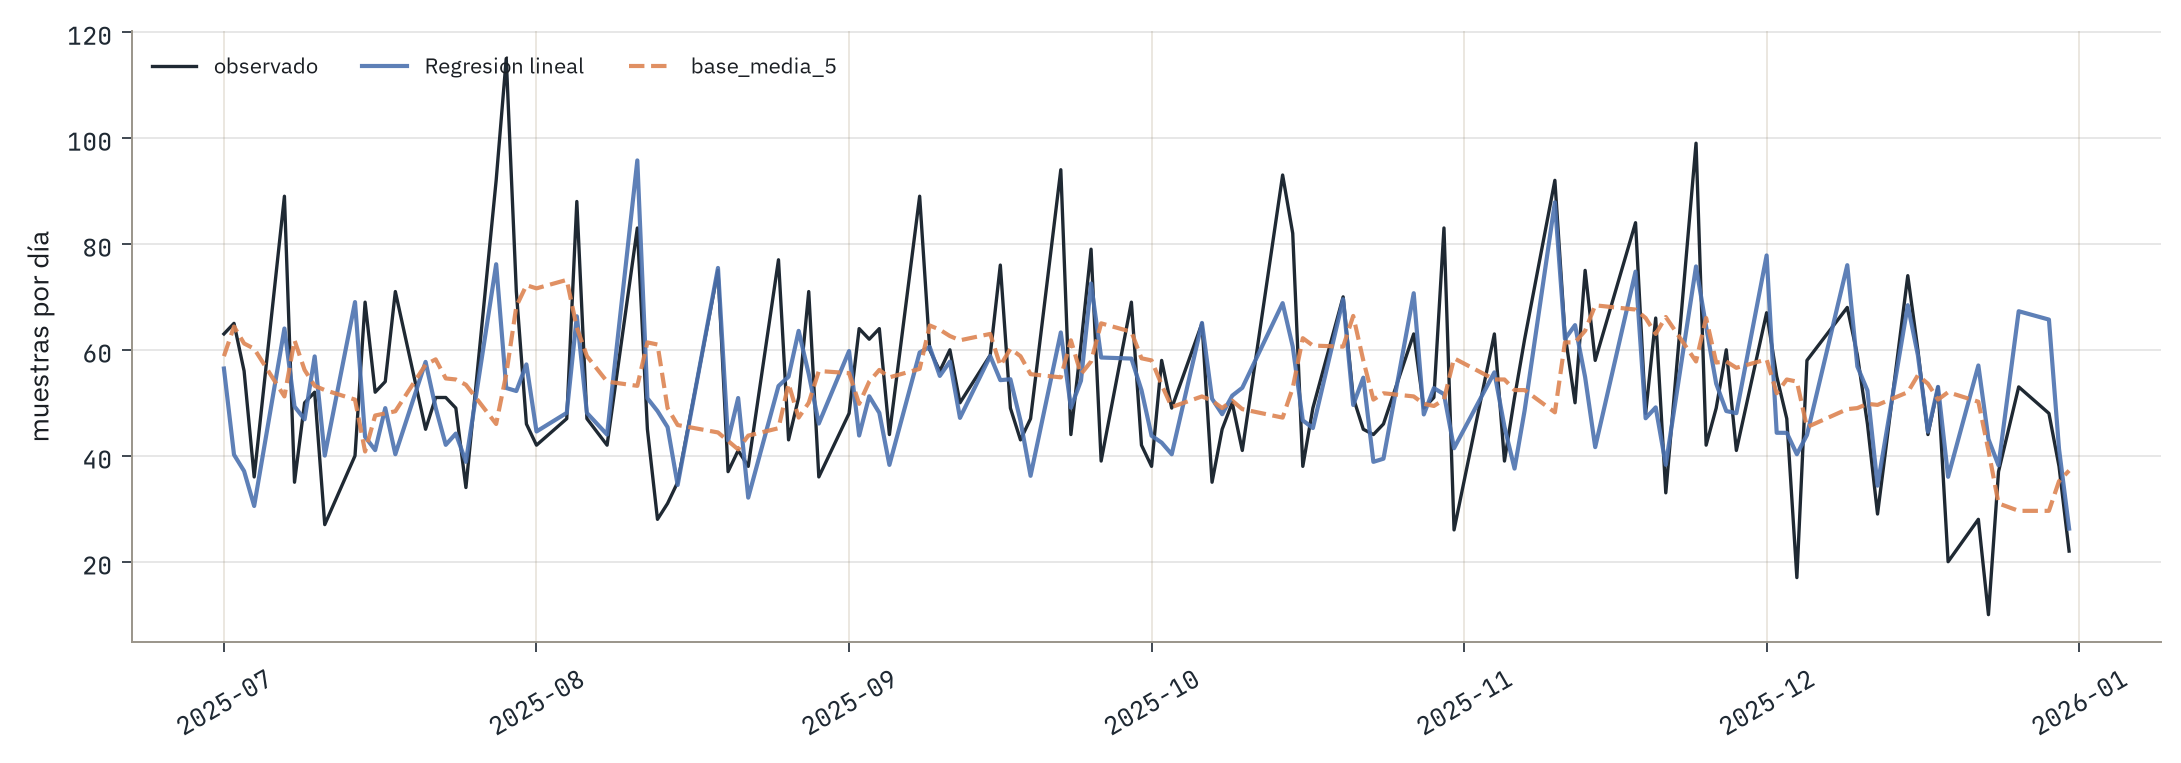
\includegraphics[width=0.85\textwidth]{04_validacion_serie.png}
\caption{Serie de validación: observado (negro), regresión lineal (azul) y
media de los cinco días anteriores (naranja). El modelo sigue los altibajos de
un día a otro, que la referencia solo suaviza, pero no alcanza los picos
aislados.}
\label{fig:reg-serie}
\end{figure}

\paragraph{Lectura operativa.} Si se acepta como tolerancia práctica un error
del \RegToleranciaOperativaPct{}\,\% de la media diaria (unas
\RegToleranciaOperativa{} muestras), el modelo queda fuera de ella en el
\RegDiasFueraPct{}\,\% de los días de validación, frente al
\RegDiasFueraReferenciaPct{}\,\% de la referencia, y su error absoluto medio es
de \RegMAEOperacion{} muestras frente a \RegMAEReferencia{}. Es una mejora
clara pero modesta, útil para planear turnos, no para fijar cupos exactos.
Finalmente, el modelo congelado (\RegModeloFinal{}, \RegVariablesModelo{}
variables tras codificar) se reajusta con entrenamiento más validación
(\RegFilasReajuste{} días) antes de abrir la prueba.
